%%%%%%%%%%%%%%%%%%%%%%%%%%%%%%%%%%%%%%%%%%%%%%%%%%%%%%%%%%%%%%%
%
%     filename  = "main.tex",
%     version   = "1.2.0",
%     authors   = "Ade Irawan",
%     email     = "adeirawan@universitaspertamina.ac.id"
%
%%%%%%%%%%%%%%%%%%%%%%%%%%%%%%%%%%%%%%%%%%%%%%%%%%%%%%%%%%%%%%%
%
% Gunakan Etc/skripsistyle.cls dan compile dengan pdflatex.
%
%%%%%%%%%%%%%%%%%%%%%%%%%%%%%%%%%%%%%%%%%%%%%%%%%%%%%%%%%%%%%%%
%
%  2020/01/06   Created              	         Ade
%  2021/02/03   tambah lembar pemisah	         Herdiansyah
%  2021/02/22   edit lembar pengesahan           Ade
%  2021/09/06   membuat lembar pemisah tidak     Dheny
%               terkena watermark
%  2022/03/29   fix indentasi lampiran di ToC    Ade
%
%%%%%%%%%%%%%%%%%%%%%%%%%%%%%%%%%%%%%%%%%%%%%%%%%%%%%%%%%%%%%%%

%------------------------------------------------------------
% Bagi pemula, skip bagian ini hingga:
% "Semua informasi penting yang diperlukan" di bawah
%------------------------------------------------------------

\documentclass{Etc/skripsistyle}
% \usepackage{showframe} % for showing the frame
\usepackage{lipsum} % for generating dummy text
\usepackage{algpseudocode} 
\usepackage{amsmath}
\usepackage{amssymb}
\usepackage{upgreek}
\usepackage{times}
\usepackage{graphicx}
\usepackage{fancyhdr}
\usepackage{sectsty}
\usepackage{indentfirst}
\usepackage{xcolor}

\usepackage{ragged2e}
\usepackage{hyperref}
\usepackage{amsthm}
\usepackage{multicol}
\usepackage{natbib} % Bibliography with APA Style
\usepackage{pdfpages}
\usepackage{background} % for adding watermark
\usepackage{longtable}
\usepackage{tabularx}
\usepackage{tabularray}

% Modify tabularray>longtblr
\DefTblrTemplate{contfoot-text}{default}{}
\DefTblrTemplate{conthead-text}{default}{}
\DefTblrTemplate{caption-tag}{default}{\tablename\hspace{0.25em}\thetable}
\DefTblrTemplate{conthead}{default}{}
\DefTblrTemplate{capcont}{default}{}
\DefTblrTemplate{caption-sep }{default}{.\hspace{0.25em}}

% untuk code
\usepackage{minted} 
\renewcommand{\theFancyVerbLine}{\sffamily \textcolor[rgb]{0.5,0.5,1.0}{\scriptsize \oldstylenums{\arabic{FancyVerbLine}}}}

% Untuk custom blok
\usepackage{tcolorbox}
\tcbuselibrary{skins,breakable}
\usetikzlibrary{shadings,shadows}
\usepackage{color}
\PassOptionsToPackage{svgnames}{xcolor}
\definecolor{codegray}{rgb}{0.5,0.5,0.5}
\newenvironment{myblock}[1]{%
    \tcolorbox[beamer,%
    noparskip,breakable,
    colframe=codegray,%
    title=#1]}%
    {\endtcolorbox}

\usepackage{geometry}
 \geometry{
 a4paper,
 left=3cm,
 top=2.5cm,
 bottom=2.5cm,
 right=2.5cm,
 }
 
 \usepackage{enumitem}
 \setlist[enumerate,1]{start=0} % only outer nesting level

\usepackage{algorithm}
\makeatletter
\renewcommand{\ALG@name}{Algoritma}
\makeatother

 \newtheorem{innercustomgeneric}{\customgenericname}
\providecommand{\customgenericname}{}
\newcommand{\newcustomtheorem}[2]{%
  \newenvironment{#1}[1]
  {%
   \renewcommand\customgenericname{#2}%
   \renewcommand\theinnercustomgeneric{##1}%
   \innercustomgeneric
  }
  {\endinnercustomgeneric}
}
\newcustomtheorem{customthm}{Teorema}
\newcustomtheorem{customdef}{Definisi}

\setlength{\footskip}{1.7cm}
%% Line Spacing
\linespread{1.103} % Jangan dihapus. Ini untuk memastikan line spacing ~15pt. Cara pengecekan: ketik "\the\baselineskip" di dalam dokumen
%% Paragraph spacing
\setlength{\parskip}{9pt}
%% Title
\usepackage{titlesec}
\usepackage{apptools}
\titleformat{\chapter}[display]{\fontsize{14}{14} \center\bfseries}{\IfAppendix{LAMPIRAN}{BAB} \thechapter}{0pt}{}{}
\titleformat{\section}
  {\fontsize{12}{12}\bfseries}{\thesection}{1em}{}
  
\titlespacing*{\chapter}{0pt}{0pt}{1em}
\titlespacing*{\section}{0pt}{0pt}{0pt}

%% Page number
\pagestyle{fancy}
\fancyhf{}
\rfoot{Universitas Pertamina \hspace{1pt}-\hspace{1pt} \thepage}

% Redefine the plain page style
\fancypagestyle{plain}{%
  \fancyhf{}%
\rfoot{Universitas Pertamina \hspace{1pt}-\hspace{1pt} \thepage}%
}

\renewcommand{\headrulewidth}{0pt}
\DeclareMathOperator*{\argmin}{arg\,min}

\hypersetup{hidelinks}
%------------------------------------------------------------
% Semua informasi penting yang diperlukan
%------------------------------------------------------------
% {Judul} dan {sub judul jika ada}. Jika tidak ada sub judul biarkan {} kosong
\title{Bukan Tugas Akhir Biasa}{}

% {Judul} dan {sub judul jika ada} dalam bahasa inggris
\titleeng{Not an Ordinary Final Project}{}

% Nama Penulis dan NIM
\author{Sebut Saja Bunga}{13203013}

% Nama Fakultas, tanpa menuliskan kata "Fakultas" di depannya
\fakultas{Sains dan Ilmu Komputer}

% Nama Program Studi, tanpa menuliskan kata "Program Studi" di depannya
\prodi{Ilmu Komputer}

% Tanggal lulus sidang (Tanggal dan bulan+tahun dipisah)
\tgllulus{17}{Agustus 2045}

% Tanggal Pengesahan oleh Pembimbing (Tanggal, bulan, dan tahun digabung)
\tglpengesahan{17 Agustus 2045}

% Tanggal pembuatan Lembar Pernyataan (Tanggal, bulan, dan tahun digabung)
\tglpernyataan{17 Agustus 2045}

% Tentukan jumlah pembimbing (1 atau 2)
\newcounter{jumlahPembimbing}\setcounter{jumlahPembimbing}{2}

% Abaikan Nama dan NIP Pembimbing kedua kalau hanya 1 pembimbing, jangan dihapus
\pembimbingsatu{Pembimbing Satu}{116xxx}
\pembimbingdua{Pembimbing Dua}{116xxx}

% Nama Ketua Program Studi dan NIP nya
\kaprodi{Kaprodi}{116xxx} % Nama dan NIP
%------------------------------------------------------------

%------------------------------------------------------------
% Watermark 
% true: gunakan watermark
% false: tanpa watermark
%------------------------------------------------------------
\newboolean{iswatermark}\setboolean{iswatermark}{false}
%--------------------------------------------------------------

%--------------------------------------------------------------
% Pemecahan suku kata
% Tambahkan kata yang pemenggalan katanya bermasalah di dokumen
% Pemenggalan suku kata dengan tanda -
% Setiap kata dipisahkan oleh spasi
%--------------------------------------------------------------
\hyphenation{me-ning-kat-kan di-tu-lis-kan me-ne-ri-ma me-la-lu-i Na-mun or-ga-ni-sa-i pe-ner-je-mah pe-me-rin-tah me-nge-na-li aug-men-ta-tion meng-gu-na-kan di-gu-na-kan learn-ing trans-fer-ing bi-sin-do se-mi-ring ber-orde sa-ling}
%--------------------------------------------------------------

%------------------------------------------------------------
% Bagi pemula, skip bagian di bawah ini hingga: "Appendices"
%------------------------------------------------------------
\begin{document}
\ActivateBG{}
\frontmatter
\upcoverpage

\lembarpengesahan
\lembarpernyataan
\abstrakind{Front/abstrakind}
\abstrakeng{Front/abstrakeng}
\katapengantar{Front/katapengantar}
\daftarisi
\daftartabel
\daftargambar

\mainmatter

%% Semua BAB
%\renewcommand{\thefootnote}{\arabic{footnote}}
\chapter{PENDAHULUAN}
\label{BAB1:pendahuluan}

\section{Latar Belakang}
 Dokumen ini menggunakan \textit{style} yang sudah didefinisikan di folder Etc/skripsityle.cls. Jangan ubah kode yang ada di \textit{file} tersebut agar dokumen ini tetap memenuhi Pedoman Laporan Tugas Akhir Universitas Pertamina. \textit{File} utama dari dokumen ini adalah \verb|main.tex|. Isi informasi yang ada di \textit{file} tersebut. Tulisan bab x dapat diisi dalam file \verb|BAB-x.tex| yang berada di dalam \textit{folder}-nya masing-masing. Jika ada gambar yang akan dimasukkan dalam suatu bab, maka gambar tersebut dalam dimasukkan dalam \textit{folder} di bab tersebut berada. Perintah \verb|\lipsum[]| digunakan untuk menghasilkan kalimat-kalimat buatan. Silahkan hapus perintah tersebut dari \textit{template}. Simbol \verb|%| digunakan untuk membuat \textit{comment}, yaitu kode yang tidak dieksekusi oleh compiler \LaTeX, sehingga dapat digunakan untuk membuat catatan atau membatalkan suatu perintah.

 Untuk membuat paragraf baru cukup pisahkan satu baris antar paragraf. Tentukan singkatan dan akronim untuk pertama kalinya digunakan dalam teks, walaupun telah didefinisikan dalam abstrak. Tulis definisinya atau nama panjangnya terlebih dahulu sebelum akronimnya. Sebagai contoh, Fakultas Sains dan Ilmu Komputer (FSIK). Singkatan yang umum seperti PERTAMINA, IEEE, ac, dc, dan rms tidak harus didefinisikan. Jangan gunakan singkatan dalam judul kecuali tidak dapat dihindari.

 Untuk membuat persamaan matematika, dapat mengacu ke tulisan berikut: \url{https://en.wikibooks.org/wiki/LaTeX/Mathematics}. 
  
\section{Rumusan Masalah}
\lipsum[7] % generate dummy sentences

% \section{Batasan Masalah}
% \lipsum[8] % generate dummy sentences
 
\section{Tujuan Penelitian}
\lipsum[9] % generate dummy sentences

\section{Manfaat Penelitian}
\lipsum[10] % generate dummy sentences
\DeactivateBG{}

\includepdf{Etc/pemisah.pdf}
\ActivateBG{}
%\renewcommand{\thefootnote}{\arabic{footnote}}
\chapter{TINJAUAN PUSTAKA}
\label{BAB2:tinjauan}

Manfaatkan penggunaan perintah \verb|\label{}| untuk menjadikan suatu bab atau subbab sebagai acuan. Untuk mengacu ke bab atau subbab itu maka gunakan perintah \verb|\ref{}|. Sebagai contoh, Bab \verb|\ref{BAB1:pendahuluan}| akan menghasilkan: Bab \ref{BAB1:pendahuluan}. Teknik yang sama juga bisa digunakan untuk mengacu ke suatu gambar atau tabel. Sebagai contoh, Gambar~\ref{fig:arsitektur} menunjukkan arsitektur dari blok \textit{Residual Networks} (ResNet) yang diambil dari \citep{2022-ade-densenet}.
\begin{figure}[h]
    \centering
    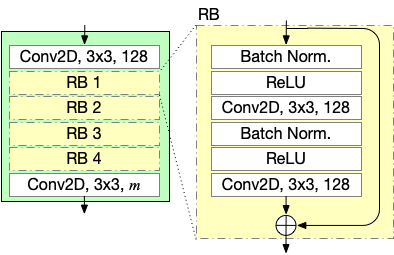
\includegraphics[scale=0.5]{BAB-2/resnet receiver.png}
    \caption{Arsitektur Blok ResNet}
    \label{fig:arsitektur}
\end{figure}

Salah satu cara untuk membuat tabel, seperti yang ditunjukkan pada Tabel~\ref{tab:test}, adalah dengan menggunakan \verb|longtblr| \citep{tabularray}.

\begin{table}[h]
    \centering
    \caption{Tabel dengan tblr}
    \label{tab:my_label}

    \begin{tblr}{lccr}
    \hline
    Alpha & Beta & Gamma & Delta \\
    \hline
    Epsilon & Zeta & Eta & Theta \\
    \hline
    Iota & Kappa & Lambda & Mu \\
    \hline
    \end{tblr}
\end{table}

\begin{longtblr}[
  caption = {Tabel yang panjang},
  label = {tab:test}
]{
  colspec = {|XX[4]|},
  rowhead = 1,
  hlines,
  row{even} = {gray9},
  row{1} = {olive9}
} 
No. & Kolom 1 \\
1  & blablabla \\
2  & blablabla \\
3  & blablabla \\
4  & blablabla \\
5  & blablabla \\
6  & blablabla \\
7  & blablabla \\
8  & blablabla \\
9  & blablabla \\
10  & blablabla \\
11  & blablabla \\
12  & blablabla \\
13  & blablabla \\
14  & blablabla \\
15  & blablabla \\
16  & blablabla \\
17  & blablabla \\
18  & blablabla \\
19  & blablabla \\
20  & blablabla \\
21  & blablabla \\
22  & blablabla \\
\end{longtblr}

\begin{longtblr}[
  caption = {Tabel Dataset Jawaban Mahasiswa},
  label = {tab:test2},
]{
  colspec = {|c|XX[1]|c|},
  rowhead = 1,
  hlines,
  row{even} = {gray9},
  row{1} = {olive9},
  % |l|,
} 
No & Nama Kolom            & Tipe Data \\  
1  & Nim                   & ordinal   \\  
2  & Jawaban pertanyaan 1  & String    \\  
3  & Jawaban pertanyaan 2  & String    \\  
4  & Jawaban pertanyaan 3  & String    \\  
5  & Jawaban pertanyaan 4  & String    \\  
6  & Jawaban pertanyaan 5  & String    \\  
7  & Jawaban pertanyaan 6  & String    \\  
8  & Nilai No 1            & nominal   \\  
9  & Nilai No 2            & nominal   \\  
10 & Nilai No 3            & nominal   \\  
11 & Nilai No 4            & nominal   \\  
12 & Nilai No 5            & nominal   \\  
14 & Total Nilai           & nominal   \\  
\end{longtblr}
\DeactivateBG{}

\includepdf{Etc/pemisah.pdf}
\ActivateBG{}
\chapter{METODE PENELITIAN}
\label{BAB3:Metode}

\lipsum[3-4] % generate dummy sentences
\DeactivateBG{}

\includepdf{Etc/pemisah.pdf}
\ActivateBG{}
\chapter{HASIL DAN PEMBAHASAN}
\label{BAB4:hasil}

\lipsum[4-5] % generate dummy sentences
\DeactivateBG{}

\includepdf{Etc/pemisah.pdf}
\ActivateBG{}
\chapter{KESIMPULAN DAN SARAN}
\label{BAB5:kesimpulan}

\section{Kesimpulan}
\lipsum[5] % generate dummy sentences

\section{Saran}
\lipsum[6] % generate dummy sentences
\DeactivateBG{}

\includepdf{Etc/pemisah.pdf}
\ActivateBG{}

%------------------------------------------------------------
% BIBLIOGRAPHY 
%------------------------------------------------------------
\begin{singlespace}
  \bibliographystyle{apalike}
  \addcontentsline{toc}{chapter}{DAFTAR PUSTAKA}
  \bibliography{referensi}
\end{singlespace}

\DeactivateBG{}

\includepdf{Etc/pemisah.pdf}
\ActivateBG{}

%------------------------------------------------------------
% Appendices
% (comment) uncomment kode di bawah ini untuk (tidak) menggunakan lampiran
% tambahkan sendiri folder-folder (lampiran) yang lain
%------------------------------------------------------------
\appendix
\Appendix{Judul Lampiran 1}
\label{lampiran1}

\section{Coding}

\lipsum[1] % generate dummy sentences

\begin{myblock}{Cara \textit{Web Scraping}}\label{Lampiran1}
\begin{minted}[xleftmargin=20pt,linenos]{python}

from bs4 import BeautifulSoup
import requests
from time import sleep
base_url = "https://www.oreilly.com/search/" + \
           "/?q=data&type=*&rows=10&page="


books = []
NUM_PAGES = 31

for page_num in range(1, NUM_PAGES + 1):
    print("souping page", page_num, ",", len(books), " found")
    url = base_url + str(page_num)
    soup = BeautifulSoup(requests.get(url).text, 'html5lib')
    
    for td in soup('td', 'thumbtext'): if not is_video(td):
        books.append(book_info(td))
        
    # give a break
    sleep(30)

def get_year(book):
    return int(book["date"].split()[1])

year_counts = Counter(get_year(book) for book in books 
                       if get_year(book) <= 2014)

import matplotlib.pyplot as plt
years = sorted(year_counts)
book_counts = [year_counts[year] for year in years] 
plt.plot(years, book_counts)
plt.ylabel("# of data books")
plt.title("Data is Big!")
plt.show()

\end{minted}
\end{myblock}

\section{Coba Masukkan Gambar}
Gambar \ref{fig:resnet} sama dengan di Bab 2.
\begin{figure}[h]
    \centering
    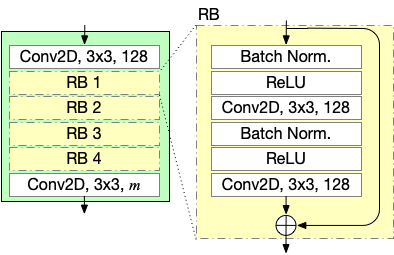
\includegraphics[scale=0.5]{BAB-2/resnet receiver.png}
    \caption{Arsitektur Blok ResNet}
    \label{fig:resnet}
\end{figure}
% \Appendix{Judul Lampiran 2}
\label{lampiran2}

\lipsum[2-3] % generate dummy sentences

\backmatter

\end{document}

%--------------------- end of file ---------------------------------------